% vim: set tw=78 sts=2 sw=2 ts=8 aw et ai:
\documentclass[12pt]{article}

\usepackage[paper=a4paper, top=2cm, bottom=3cm, left=2.5cm, right=2.5cm]{geometry}

\usepackage{ucs}
\usepackage[utf8x]{inputenc}
\usepackage[english]{babel}
%\usepackage{hyperref}	  % use \url{http://$URL} or \href{http://$URL}{Name}
\usepackage{underscore}	  % underscores need not be escaped
\usepackage{subfigure}
\usepackage{verbatim}
\usepackage{float}
\usepackage{booktabs}     % professional tables
\usepackage{hyperref}
\usepackage{amsmath}
\usepackage[export]{adjustbox}
\usepackage{algorithm}
\usepackage{algpseudocode}

% Support for including graphics
\usepackage{graphicx}
\DeclareGraphicsExtensions{.pdf,.png,.jpg}
\graphicspath{ {./img/} }

\title{Historic Events Identification in Texts}

\author{Tiberiu Popa\\
Automatic Control and Computers Faculty\\
University POLITEHNICA of Bucharest\\
Splaiul Independenței nr. 313, Bucharest, Romania \\
\emph{tiberiu.popa@cs.pub.ro}}

\date{\today}

\begin{document}

\maketitle

\begin{abstract}
% This file contains the abstract of the thesis

Here goes the abstract about \project. Lorem ipsum dolor sit amet, consectetur adipiscing elit. Aenean aliquam lectus vel orci malesuada accumsan. Sed lacinia egestas tortor, eget tristique dolor congue sit amet. Curabitur ut nisl a nisi consequat mollis sit amet quis nisl. Vestibulum hendrerit velit at odio sodales pretium. Nam quis tortor sed ante varius sodales. Etiam lacus arcu, placerat sed laoreet a, facilisis sed nunc. Nam gravida fringilla ligula, eu congue lorem feugiat eu.

\end{abstract}

\section{Introduction}
\label{sec:introduction}
% vim: set tw=78 sts=2 sw=2 ts=8 aw et ai:

Traditionally, historic events have been analyzed from the perspective of carefully selected texts, deemed historically significant. This has allowed historians to paint accurate descriptions of important events in our history, from a variety of perspectives: the underlying motives and actions that lead to a particular event, the narrative of the event (as a sequence of minor events) and the influence that said event has had on humans and their culture. In recent times, the sources for historians have diversified due to advancements in technology, but written texts still remain invaluable for this task.

However, as proven by the recent advent of the field of culturomics, introduced in \newcite{Michel14012011}, there is much to be learned by analyzing the large collections of books available in electronic form. More specifically, by seeking patterns in the time series of the frequency of a given word as a function of the year, it is possible to make clever observations in fields such as linguistics (grammar evolution), but also in areas pertaining to social sciences, such as collective memory, adoption of technology and censorship.

This paper delves deeper into the implications of this approach to the analysis of historic events. Thus, the purpose is to devise a model that can be used for the identification of important events in texts, by using quantitative data collected from millions of books instead of relying on understanding a few select texts.


\section{Related Work}
\label{sec:relatedwork}
% vim: set tw=78 sts=2 sw=2 ts=8 aw et ai:

In \cite{Michel14012011}, Michel et al. have laid the foundation of culturomics, i.e. the quantitative analysis of culture. Thus, using a corpus of over 5 million books, i.e. about $4 \%$ of all the books ever published, they have managed to computationally investigate cultural trends. This meant that now social sciences have a complementary approach available to the traditional analysis usually employed.

The essential ingredient of the study was of course the large corpus used. Without it, it would have been very difficult to select an unbiased sample of texts that yielded significant results. The exact same corpus, Google Books Ngram Corpus, shall be used in this paper, so I'll go into greater detail about its structure. Thus, over 15 million books have been digitized for the Google Books project using optical character recognition (or OCR). The main languages used in the books are English, French, Spanish, German, Chinese, Russian and Hebrew. The resulting corpus was then filtered to increase its quality in two regards. First of all, they used a clever algorithm to estimate the accuracy of the OCR for any given book and set a threshold on the quality, generally around $50 - 80 \%$, depending on the language. Secondly, the metadata for each book was collected from various sources, but many times conflicts would appear. Therefore, they also removed books that had low accuracy of metadata referring to the date of publication and to the language. In the end, about 5 million books remained as a basis for the Ngram Corpus.

Instead of providing access to the raw books, due to copyright restrictions, the Google Books Ngram Corpus actually consists of n-gram statistics for sequences of up to 5 words. Thus, for each n-gram, the following information is available for any given year: the number of times the n-gram has appeared in books written in that year, the number of pages in which it appeared and the number of volumes in which it appeared. Since the number of books written each year is constantly increasing, one can also derive more informative measures from this data. One way to do this would to be to normalize the statistics. For example, one can divide the first one by the total number of n-grams that appeared in books written in that year. The last measure presented is also used by Google Books Ngram Viewer \cite{ngramviewer}, a web application for visualizing the time series for one or more n-grams.

The applications of culturomics are numerous, the most obvious of which would be in linguistics. It has been found that the English lexicon has about 1 million words, while the largest dictionary lists only $350,000$ of them. Also, one can use the data to study the evolution of grammar, such as the transition of verbs from irregular to regular or vice versa.

However, the most interesting applications lie in the social sciences. For example, by studying the time series of various inventions, one can analyze the rate at which technology is adopted into widespread use. Other examples are closely related to historic events. Firstly, Nazi censorship has left visible marks on the published books and censored individuals can be easily identified by comparing their n-grams during the Nazi regime with those in the adjacent periods of time. Secondly, one can deduce from the plot associated with influenza when the most devastating flu pandemics have occurred: they correspond to the peaks in the time series. The same idea works in the case of the American Civil War, using the graphs of "the North" and "the South".

This kind of analyses can also be applied to more recent corpora, such as news archives. In \cite{leetaru11culturomics}, Leetaru has used data from the Summary of World Broadcasts to analyze events such as the Arab Spring and ethnic conflicts such as the one that occurred in Serbia in the 1990s. Another more spectacular application is determining the location of Bin Laden's hideout by analyzing cities that appear in the same article with his name, the result being off by less than 200 kilometers. Although not relevant specifically to the current research, it is a further proof of the utility of culturomics in analyzing historic events.

This paper will focus on peaks of n-gram time series, such as those of influenza, as previously mentioned. However, instead of examining particular cases, I shall analyze a significant portion of the time series by running a peak detection algorithm. The resulting data shall then be used for characterizing the underlying historic events.


\section{Historic Events Model}
\label{sec:model}
% vim: set tw=78 sts=2 sw=2 ts=8 aw et ai:

\subsection{Corpus, Smoothing and Historical Relevance}

The analysis shall be based on the Google Books Ngram Corpus and the time series it provides for each word, mapping the year of publishing to the normalized frequency of the n-gram in books written in that year. The time spanned by the series is between $1500$ and $2008$. Let us denote the time series for a given word $w_i$ by $\left\{ s_{i, t} \right\}_{t = 1500}^{2008}$. In order to mitigate the effect of noise on the data, we instead use the smoothed series with window size $k$, given by:

\begin{align}
\label{eq:smooth-series}
u_{k} \left( i, t \right) = \frac{\sum_{d = -k}^{k} s_{i, t + d}}{2k + 1}.
\end{align}

The value of this window size was empirically chosen to be $k = 2$.

The data provided by the Google Books Ngram Corpus is immense (about 30 GB), so trying to identify historic events using all of the raw data seems to be an intractable problem. Thus, a better idea is to model the historical relevance of an n-gram in a given year on a discrete scale, for example the integers in $\left[ 0, 10 \right]$, where $0$ would reflect the n-gram's lack of importance and $10$ would reflect a year-defining n-gram. Due to the implicit localized nature of historic events, any given n-gram should attain historical relevance only within a small time frame. Thus, most of the entries in the reduced time series should be $0$, leading to a highly sparse representation. Therefore, not only is this transformation useful from a practical point of view (it drastically reduces the computational resources required for the analysis), but it also has theoretical arguments that it maps well to the task of historic events identification.

\subsection{Historical Relevance Algorithms}
\label{sec:historical-relevance-algorithms}
% vim: set tw=78 sts=2 sw=2 ts=8 aw et ai:

In order to explain the algorithms used for determining historical relevance, I shall first analyze a typical time series, using as example a word that carries a heavy influence on history: war.

\begin{figure}
\centering
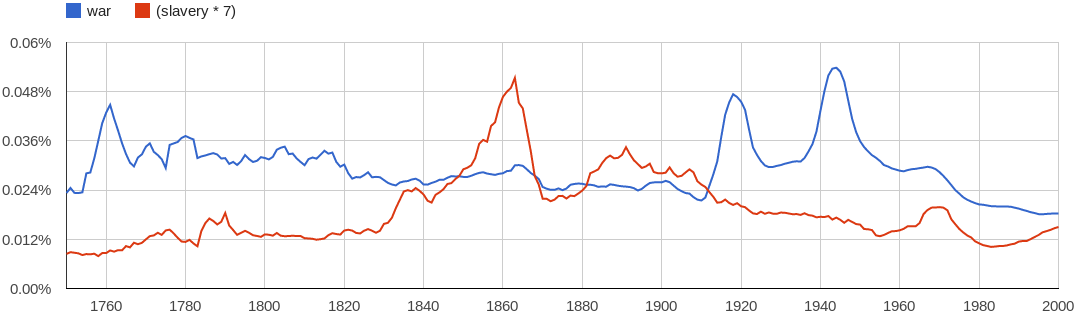
\includegraphics[max size={\textwidth}{\textheight}]{war-series}
\caption{Ngram time series for war}
\label{fig:war-series}
\end{figure}

Taking a look at \autoref{fig:war-series}, the first feature of the plot that can be noticed is the presence of several well-defined peaks. One can immediately make the connection of the three obvious peaks with historic events: the first one, between $1755$ and $1765$, corresponds to the Seven Years' War, which involved most of Europe, North America, Central America, West Africa and India; the second one, between $1910$ and $1926$, is clearly caused by World War I, which was centred in Europe and involved around 70 million military personnel; the third one, between $1936$ and $1953$, is determined by World War II, which was fought by most of the planet's nations and resulted into upwards of 50 million casualties.

However, a closer inspection reveals the presence of further peak-like shapes, some of which can be identified with major wars in history. Between $1775$ and $1783$ took place the American Revolutionary War, which not only involved Great Britain and the United States, but also France, Netherlands and Spain. Between $1860$ and $1871$ one can note another peak most probably corresponding to the American Civil War, which had the abolition of slavery as one of its goals. More recently, between $1961$ and $1978$, there is a shape vaguely resembling a peak most likely generated by the Vietnam War, fought between North Vietnam and its communist allies on the one side and South Vietnam and the United States on the other. From these observations, it is clear that the analysis of only one n-gram, war, cannot be solely used to determine the major wars that have taken place in our history. The shape of a singular plot can only reveal so much information, but by determining historical relevance for different n-grams and correlating the results, one can viably get a picture of a historic event.

\begin{figure}
\centering
\includegraphics[max size={\textwidth}{\textheight}]{comparative-series}
\caption{Ngram time series for atomic, trench and slavery}
\label{fig:comparative-series}
\end{figure}

As a prime example of the above idea, \autoref{fig:comparative-series} presents a comparative analysis of the following 3 n-grams: atomic, trench and slavery. Note that I have taken the freedom to scale the three plots for easier visualization, as in the end it is only the shape of the graph that is under scrutiny. One can notice three surges in the frequency time series. Firstly, slavery has a very sharp triangular peak between $1842$ and $1871$, which includes the American Civil War, known for the fact it had slavery as a core issue. Secondly, trench has a significant peak between $1911$ and $1925$, corresponding to World War I, known for the heavy use of trench warfare. Lastly, atomic also has a wide peak between $1939$ and $1972$, motivated by the development of the atomic bomb, its use in World War II and its potential use in the Cold War.

For this analysis to be tractable on the large amounts of data available in the corpus, one must come up with an algorithm for peak detection. It has to be not only reliable, but also has to run fast enough so it can cope with the limited amount of resources. The trade-off that can be made in this situation is between complexity of the peak detection algorithm and the amount of data that can be actually processed. At one extreme, if the algorithm is too simple, it can process all the data, but the results will probably be of inferior quality. At the other, if the algorithm is too complicated, it can only process a negligible portion of the corpus, so again the results are likely to be mediocre. Another decision to be made here is selecting the corpus subset that is left out. The intuitive solution is to leave out the least frequent n-grams, the heuristic being that rare words are pretty unlikely to be connected with a major historic event.

A further requirement for the algorithm is the capability of meaningfully characterizing a peak. Thus, besides determining the period of time that a peak occurred, it also needs to quantitatively measure the historical relevance of that peak. In the example of the n-gram war, the three large peaks should be assigned a high historical relevance. In regard to the other three lesser peaks, it is debatable whether the algorithm should even detect them, but in case it does, they should be assigned a low historical relevance. Furthermore, the value of the historical relevance needs not be constant over the entire peak. Instead, advanced schemes can use a variable historical relevance, perhaps assigning more to the center of the peak and less to the outskirts of the peak.

\subsubsection{Double Change Peak Detection}

Arguably the simplest way of detecting peaks is by making use of the fact that peaks usually consist of a period of abrupt increase, followed by another period of abrupt decrease. A computationally inexpensive method for doing this is detecting periods of time marked by a double change of the time series in the same direction, either increasing or decreasing.

Formally, we say that a time series $\left\{ s_{i, t} \right\}$ suffers a double increase of magnitude $x \in \left[ 0, 1 \right)$ at time $t$ if:

\begin{align}
\label{eq:double-increase}
s_{i, t} > \left( 1 + x \right) s_{i, t - 1} \textrm{ and } s_{i, t + 1} > \left( 1 + x \right) s_{i, t}.
\end{align}

Similarly, we say that a time series $\left\{ s_{i, t} \right\}$ suffers a double decrease of magnitude $x \in \left[ 0, 1 \right)$ at time $t$ if:

\begin{align}
\label{eq:double-decrease}
s_{i, t} < \left( 1 - x \right) s_{i, t - 1} \textrm{ and } s_{i, t + 1} < \left( 1 - x \right) s_{i, t}.
\end{align}

One problem that may appear with these definitions is that, for example, during the ascent part of the peak, at often times the increase rate will randomly dip below a certain threshold, causing the algorithm to miss a valuable information. To this end, I have also introduced the notion of single increase of magnitude $x \in \left[ 0, 1 \right)$:

\begin{align}
\label{eq:single-increase}
s_{i, t} &> \left( 1 + 2x \right) s_{i, t - 1}.
\end{align}

Similarly, the notion of single decrease of magnitude $x \in \left[ 0, 1 \right)$ is defined as follows:

\begin{align}
\label{eq:single-decrease}
s_{i, t} &< \left( 1 - 2x \right) s_{i, t - 1}.
\end{align}

As can be noticed, the latter two notions use a factor of $2x$ in the formulas instead of the $x$ used in the double change formulas. The reasoning behind this is that although we don't want to miss any potential peaks, single changes in the time series can sometimes not be part of a peak. Therefore, I made it harder for single changes to achieve a certain magnitude, while still making sure that the original problem was also solved.

The magnitude $m_{i, t}$ of the change around a point $t$ in a time series $\left\{ s_{i, t} \right\}$ is defined as the maximum between the magnitude of the double change and the magnitude of the single change at that point. From this, the historical relevance is computed as follows:

\begin{align}
\label{eq:double-change-relevance}
r_{i, t} &= \min \left( \left\lfloor 10 m_{i, t} \right\rfloor, 9 \right).
\end{align}

The relevance value is thus an integer proportional to the magnitude $m_{i, t}$. However, an artificial cap has been placed on this value, because n-grams can grow very fast, especially when a new term is born. This has the positive effect of not overemphasizing the exploding word.

\subsubsection{Linear Model Peak Detection}

Drawing on the previous idea of periods of abrupt increase and decrease, one can also use a linear model for approximating portions of the time series. The core of this approach is to fit lines to the graph of the time series using linear regression, by considering larger and larger intervals until the error rises above a given threshold.

\begin{algorithm}

\begin{algorithmic}[1]
\For { $i \in 1 \to \left| \textrm{Words} \right|$ }
    \For { $t \in 1500 \to 2008$ }
        \State $s_{i, t} = \frac{s_{i, t} - \mu_i}{\sigma_i}$
    \EndFor
\EndFor
\For { $i \in 1 \to \left| \textrm{Words} \right|$ }
    \State $u \gets 1500$
    \For { $t \in 1501 \to 2008$ }
        \State $a, b, err \gets \textrm{lm} \left( \left\{ s{i, k}_{k = u}^t \right\} \right)$
        \Comment { Parameters and error of the model $y = ax + b$ }
        \If { $\log(err) >= -5$ }
            \State $m_i \left( u, t \right) \gets 2 \cdot \left( 3 + \log \left| a \right| \right)$
            \State $u \gets t$
        \EndIf
    \EndFor
\EndFor
\end{algorithmic}

\caption{Linear Model Peak Detection Algorithm}
\label{alg:linear-model}

\end{algorithm}

As can be noticed in Algorithm \autoref{alg:linear-model}, the series is first transformed using the standard score, such that, after the transformation, its mean shall be 0 and its variance 1. This is a standard step used for preparing the data for linear regression. Upon finding a maximal interval fitted by a line within a small error, the magnitude of the change on that interval is defined as a linear function of the logarithm of the slope (actually, the absolute value of that slope, since it can also be negative). This choice reflects a wide range of values that the slope can take, forming a sort of heavy-tailed distribution. Taking the logarithm of the slope cancels the effect of the heavy tail and allows for interesting statistics to be collected.

Since taking logarithms eliminates the possibility of ridiculously high magnitudes, the historical relevance for $w_i$ can simply be computed as follows:

\begin{align}
\label{eq:linear-model-relevance}
r_{i, t} &= \max \left( \left\lfloor m_{i, t} \right\rfloor, 0 \right).
\end{align}

\subsubsection{Gaussian Model Peak Detection}

Another completely different idea for peak detection is to notice that peaks are usually shaped like a Gaussian distribution, i.e. they are bell-shaped. So, let's consider a time interval $\left[ l, r \right] \subseteq \left[ 1500, 2008 \right]$ and the time series for some word $w_i$ on that interval, $\left\{ s_{i, t} \right\}_{t=l}^{r}$. Since we want to approximate the series by a normal distribution, it should be probably normalized to that it sums to 1. However, this is not enough, since a Gaussian has an infimum of 0, while a peak can be offset by a significant value. This offset is of course computed as the minimum value of the time series on the given interval. Thus, we define the normalized time series $\left\{ g_{i, t} \right\}_{t=l}^{r}$ as:

\begin{align}
\label{eq:gaussian-normalization}
g_{i, t} &= \frac{s_{i, t} - \min_{p \in \overline{l, r}} s_{i, p}}{\sum_{q = l}^{r} \left( s_{i, q} - \min_{p \in \overline{l, r}} s_{i, p} \right)}.
\end{align}

This is approximated by a normal distribution $N \left( \mu, \sigma \right)$ with the following parameters:

\begin{align}
\label{eq:mu-gaussian-model}
\mu &= \frac{\sum_{t=l}^{r} g_{i, t} t}{r - l + 1}, \\
\label{eq:sigma-gaussian-model}
\sigma^2 &= \frac{\sum_{t=l}^{r} g_{i, t} \left( t - \mu \right)^2}{r - l + 1}.
\end{align}

In order to compute the similarity between $g_{i, t}$ and $N \left( \mu, \sigma \right)$, a variation on the earth mover's distance \cite{rubner98metric} shall be used. Although the former probability distribution is discrete, while the latter is continuous, we shall nonetheless assume that the latter is also discrete by considering only its values in the points $t \in \overline{l, r}$.

\begin{algorithm}

\begin{algorithmic}[1]
\Require $l \geq 1500, r \leq 2008$
\State $acc \gets 0$
\State $distance \gets 0$
\For { $t \in l \to r$ }
    \State $acc \gets acc + g_{i, t} - \frac{1}{\sqrt{2 \pi} \cdot \sigma} \cdot \exp \left( - \frac{\left( t - \mu \right)^2}{2 \sigma^2} \right)$
    \State $distance \gets distance + \left| acc \right|$
\EndFor
\State \Return $distance$
\end{algorithmic}

\caption{Earth Mover's Distance Algorithm}
\label{alg:emd}

\end{algorithm}

The well-known Algorithm \autoref{alg:emd} is based on the idea of treating the value of a probability distribution at a certain point as the amount of dirt found at that distance. Then the distance between two distributions is equal to the minimum amount of work required for transforming a distribution into the other, where work is defined as the amount of dirt moved times the distance it is moved. In general, this is equivalent to the assignment problem, so it can be solved using the Hungarian algorithm. However, in the one-dimensional case, the greedy algorithm presented above works.

In the case of modeling peaks with Gaussian distributions, unfortunately we have to consider all possible intervals $\left[ l, r \right] \subseteq \left[ 1500, 2008 \right]$, which leads to quadratic complexity in the number of invocations of the earth mover's distance algorithm, which is itself linear in the length of the interval. Overall, this leads to a total $O \left( \max(r) - \min(l) \right)^3$ complexity. In order to bring this down an order of magnitude, one needs a heuristic to decide if a probability distribution even remotely looks like a Gaussian bell. To this end, I have chosen to use kurtosis:

\begin{align}
\label{eq:kurtosis}
\gamma_2 &= \frac{\mu_4}{\sigma^4} - 3.
\end{align}

Here, $\mu_4$ is the fourth moment about the mean:

\begin{align}
\label{eq:4th-moment}
\mu_4 &= \frac{\sum_{t=l}^{r} \left( g_{i, t} - \mu \right)^4}{r - l + 1}.
\end{align}

As evidenced in \cite{balanda88kurtosis}, in the case of symmetric distributions, kurtosis can be viewed as an approximate measure of peakedness, with the normal distribution having a kurtosis of 0. Furthermore, kurtosis can be computed, with trivial preprocessing of partial sums, in constant time for any interval $\left[ l, r \right]$. Thus, by imposing a tight limit on the absolute value of the kurtosis, such as $0.05$, the complexity of processing a time series drops heavily and thus one can process even more of them in total.

After that, from the remaining intervals we select the ones that have an earth mover's distance to their corresponding Gaussian distributions lower than $0.3$. A potential problem that can appear is that the intervals may intersect. This can be avoided by first sorting the intervals in increasing order of the earth mover's distance and then processing them one by one. Intervals that intersect previously processed ones are simply ignored, which both ensures that the intervals are disjoint and that only the highest quality peaks are chosen.

Now we compute the magnitude of the change corresponding to an interval $\left[ l, r \right]$ as the percentage with which the Gaussian peak increases from its smallest value to its largest value. The minimum value is computed as a statistic from the original series, while the largest value is derived from the largest value of the Gaussian distribution (which occurs exactly at its mean):

\begin{align}
\label{eq:gaussian-magnitude}
m_i \left( l, r \right) &= \frac{N \left( \mu, \sigma \right) \left( \mu \right) \cdot \sum_{q = l}^{r} \left( s_{i, q} - \min_{p \in \overline{l, r}} s_{i, p} \right)}{\min_{p \in \overline{l, r}} s_{i, p}}.
\end{align}

One way to define historical relevance in this case is to assign it a constant value on the interval, proportional to the magnitude:

\begin{align}
\label{eq:gaussian-model-constant-relevance}
r_{i, t} &= \left\lfloor 10 \cdot \min \left( m_i \left( l, r \right), 1) \right) \right\rfloor, \, \forall t \in \left[ l, r \right].
\end{align}

An alternative way is to assign variable relevance, such that it also forms a Gaussian bell. The formula, that also includes a widening parameter $w \in \left[ 1, \infty \right)$, is as follows:

\begin{align}
\label{eq:gaussian-model-variable-relevance}
r_{i, t} \left( w \right) &= \left\lfloor 10 \cdot \min \left( m_i \left( l, r \right), 1) \right) \right\rfloor \cdot \frac{N \left( \mu, w \sigma \right) \left( t \right)}{N \left( \mu, w \sigma \right) \left( \mu \right)}, \, \forall t \in \left[ l, r \right].
\end{align}

One can note that when $w \to \infty$, \autoref{eq:gaussian-model-variable-relevance} actually converges to \autoref{eq:gaussian-model-constant-relevance}. The idea behind the parameter $w$ is that both extremes are likely to give poor performance: for $w = 1$, too little relevance is assigned to the tails of the distribution, while for $w \to \infty$ too much relevance is assigned to the tails of the distribution. By considering intermediate values one is likely to obtain higher quality results.

\subsubsection{Graphical Analysis}

\begin{figure}
\centering
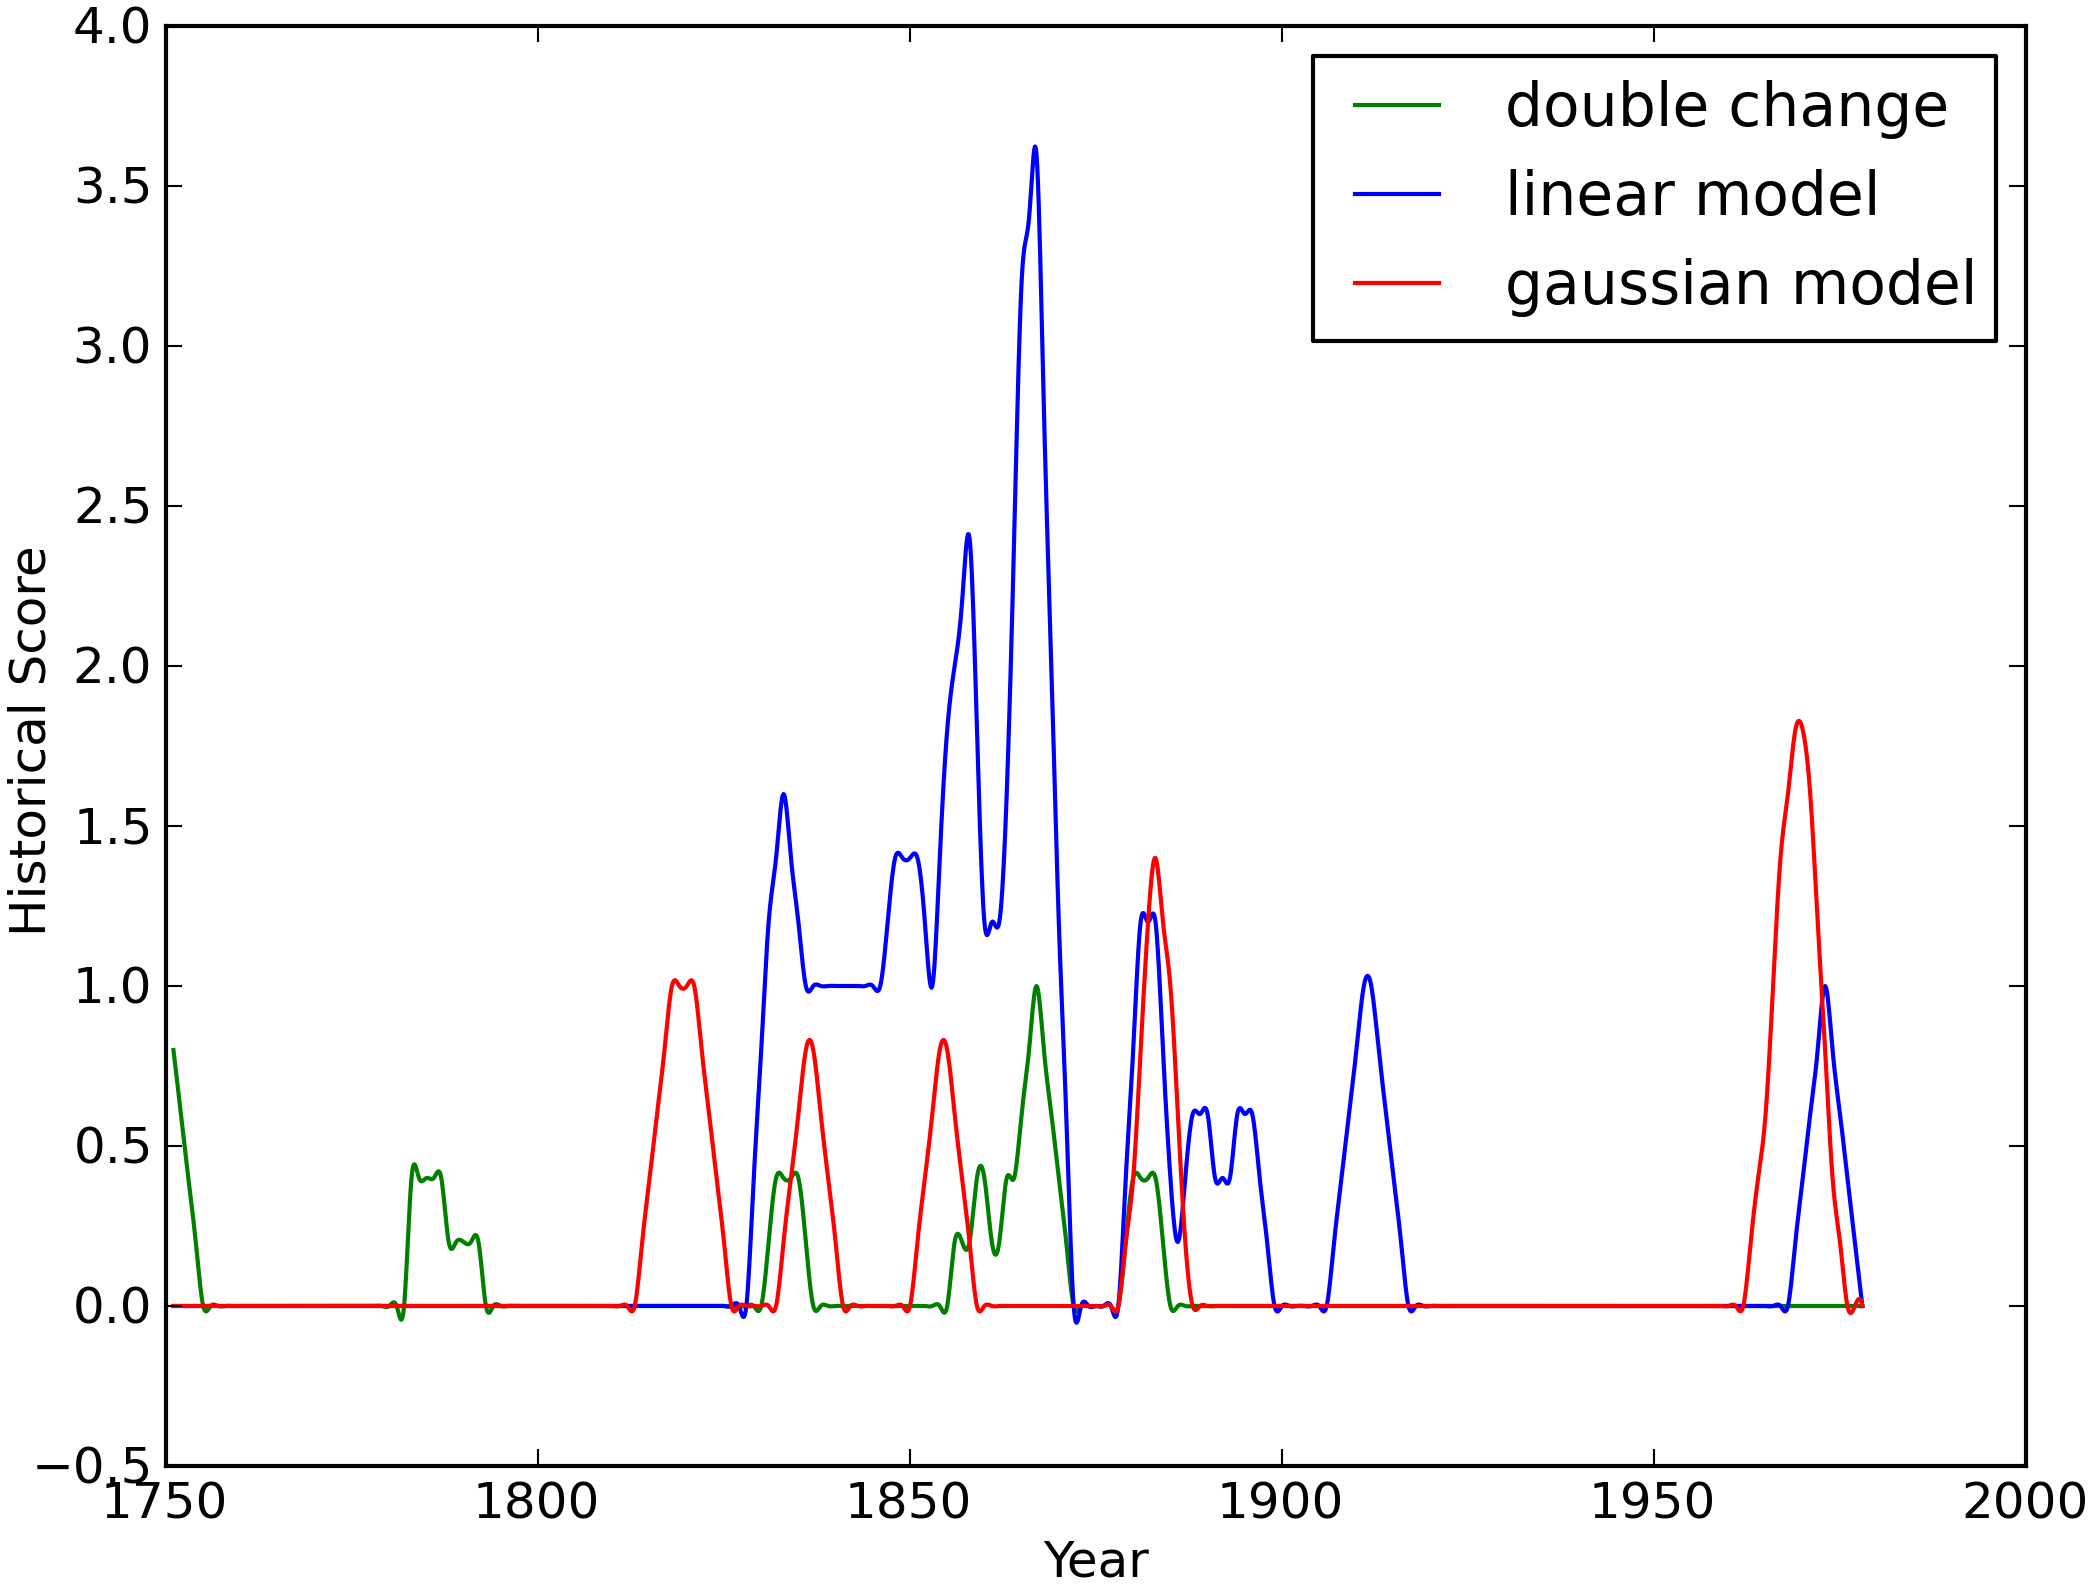
\includegraphics[max size={0.8 \textwidth}{0.8 \textheight}]{slavery-relevance}
\caption{Historical relevance of slavery}
\label{fig:slavery-relevance}
\end{figure}

Of the three algorithms, it cannot be said that one of the them performs the best at detecting and characterizing peaks. However, with the help of an example such as \autoref{fig:slavery-relevance}, one can point the strengths and weaknesses of each of them (for the Gaussian model, I have used the widening parameter $w = 2$). As it could be seen in \autoref{fig:comparative-series}, slavery has had two important "historic peaks": the first, between $1842$ and $1871$, includes the American Civil War, while the second, between $1964$ and $1979$, includes the African-American Civil Rights Movement.

The first peak is detected by all three algorithms. Since it is triangular in shape, the best detection is performed by the linear model algorithm, since it can be approximated pretty well with 2 lines. The other two algorithms also detect activity in this period, but in 2 distinct intervals. Although it seems the results are worse, it can be noted that the second interval detected by the Gaussian model is centered around the American Civil War. The conclusion that can be drawn from this example is that although the linear model is better at detecting triangular peaks, the Gaussian model does a better job at identifying the high point that probably corresponds to a historic event. The double change model is significantly worse than the other two, since it more likely assigns relevance to the tails of the triangle, rather than to the peak.

The second peak is detected only by the last two algorithms. Although both reasonably identify the peak, the Gaussian model performs better by considering a slightly larger interval. This is to be expected, as the peak is roughly bell-shaped.

Lastly, the double change model also detects a minor peak centered around $1790$. In that period, the Constitution of the United States was drafted, and one if its highlights was the Three-Fifths Compromise, which stated that for representation purposes, slaves counted as only three-fifths of a person. Thus, although theoretically inferior to the other two algorithms, the double change model has the capability of detecting less important historic events.


\subsection{Historically Relevant Documents and Topic Models}

For each year $t \in \left[ 1500, 2008 \right]$, we build its historically relevant document $d_t$ as follows: we include each $w_i$ (that satisfies $r_{i, t} > 0$) exactly $r_{i, t}$ times. Topic models seem most suitable for automatically analyzing the data, as they are designed for discovering the hidden thematic structure in document collections \newcite{Blei:2012:PTM:2133806.2133826}. The specific algorithm used in this paper is the Latent Dirichlet Allocation (LDA) \newcite{Blei:2003:LDA:944919.944937}. Upon applying it to the historically relevant documents, ideally the topics found by the algorithm should represent the types of historic events, while the topic distribution for any given year should represent the underlying historic events. However, what ends up happening is that recurrent themes for consecutive years are grouped into a topic. While this still needs the intervention of a human to interpret the keywords pointing either to historic events or to cultural trends, the data that must be analyzed is significantly smaller in size.


\section{Implementation}
\label{sec:implementation}
\chapter{Implementation}
\label{chapter:implementation}

\begin{figure}
\centering
\includegraphics[max size={\textwidth}{\textheight}]{modules}
\caption{Modules diagram}
\label{fig:modules}
\end{figure}

The implementation revolves around a few highly decoupled modules, who communicate with each other through data stored on the disk, as shown in \autoref{fig:modules}. The data is stored in various formats, which I will describe now. First, there is the Google Books Ngram Corpus, made freely available by Google, stored in comma-separated values (CSV) format. Second, I need to process a lot of data fast, so the obvious choice is to create a Binary Ngram format. This format requires the use of not one but three files: a main file that stores metadata for each possible n-gram, such as offsets in the next two files at which to find further information; a words file that stores all the n-grams as one long string; a time file that stores all words' time series. Third, the historically relevant documents are stored in CSV format. Fourth and finally, the topic data is generated by an external tool and is stored in a combination of CSV and text files.

The modules deal with transforming the data from and to various formats. The Binary Ngram Module is tasked with reading and writing the files used in the Binary Ngram format. Also, it includes a trivial CSV parser for the Google Books Ngram Corpus and is fully implemented in C/C++. The Historical Relevance Module implements all the algorithms discussed in \labelindexref{Section}{sec:historical-relevance-algorithms}, relying on the Binary Ngram Module to access the data as fast as possible, and its main purpose is to create the historically relevant documents. Again, this part is also implemented in C/C++. The Topic Modeling Module uses an external tool, the Stanford Topic Modeling Toolbox \cite{stanfordtmt}, called using a Scala script, to create a topic model from the historically relevant documents. The Processing Module helps understand the data obtained at various stages of the process. For example, it transforms the output of the Historical Relevance Module to a graphical form, allowing for comparison with the original time series. Furthermore, it analyzes the output of the Stanford Topic Modeling Toolbox to create a cleaner representation of which topics correspond to which time intervals. This final module is written in Python.


\section{Results}
\label{sec:results}
% vim: set tw=78 sts=2 sw=2 ts=8 aw et ai:

Topic models specify a mixture of topics for each historically relevant document and thus for each year. The analysis of all variants of relevance has shown that only rarely does a year fail to have a dominant topic (over $50 \%$), so only the most likely topic for each year shall be considered.

\begin{figure*}[ht]
\centering
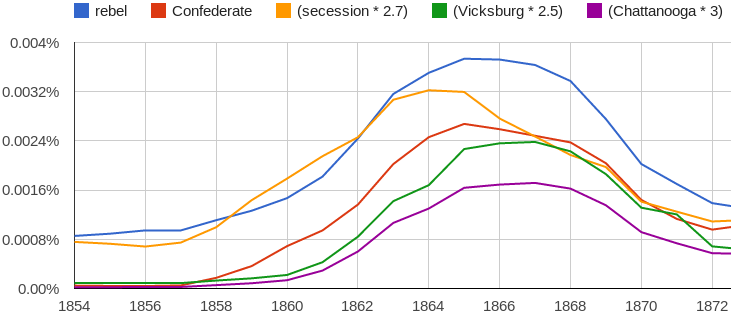
\includegraphics[max size={0.7 \textwidth}{0.7 \textheight}]{civil-war-related-series}
\caption{Ngram time series related to the American Civil War}
\label{fig:civil-war-related-series}
\end{figure*}

Though seemingly the weakest model, the double change algorithm has generated some of the most accurate topics for certain periods of time. For example, the topic for the years $1858$ to $1864$ and $1867$ to $1868$ is composed of the following main words: rebel, confederate, wolff, mcclellan, schleswig, secession, ich, vicksburg, rebels, chattanooga, die, sherman, doge, nicht, wedgwood, holstein, longstreet, gen, flax and der. A lot of these words relate directly to the American Civil War (see Figure~\ref{fig:civil-war-related-series}), providing a high degree of confidence that the model has successfully detected this important event in history.

\begin{figure*}[ht]
\centering
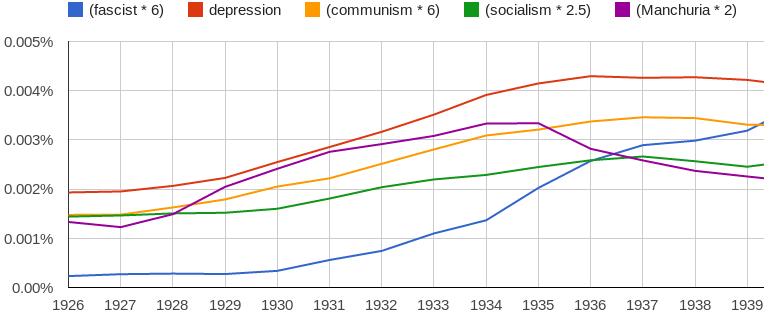
\includegraphics[max size={0.7 \textwidth}{0.7 \textheight}]{pre-ww2-related-series}
\caption{Ngram time series related to the pre World War II period}
\label{fig:pre-ww2-related-series}
\end{figure*}

For the linear model peak detection, the time period under consideration spans from $1932$ to $1936$, filled with events that foreshadowed World War II. The detected topic consists of fascist, adjustment, federal, depression, rubber, communism, collective, pact, medieval, vitamin, broadcasting, reconstruction, alpha, recovery, radio, employers, socialism, communists, tomorrow and manchuria. Unlike the case of the American Civil War, there is no underlying important event that could cause the topic to converge. Nonetheless, the selected words, the most relevant of which are shown in Figure~\ref{fig:pre-ww2-related-series}, do a good job of painting an accurate image of that period.

\begin{figure*}[ht]
\centering
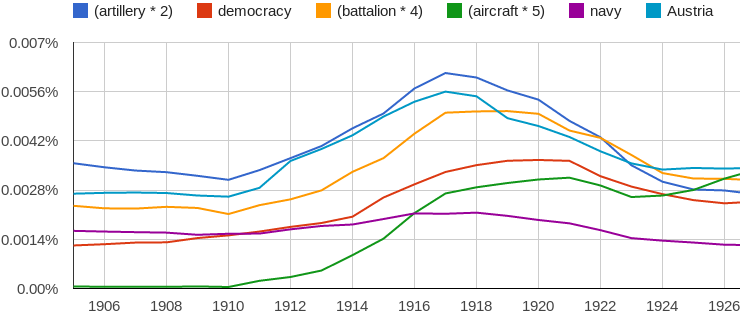
\includegraphics[max size={0.7 \textwidth}{0.7 \textheight}]{ww1-related-series}
\caption{Ngram time series related to World War I}
\label{fig:ww1-related-series}
\end{figure*}

For the last model, Gaussian model peak detection, the interval between $1916$ and $1920$ has a topic consisting of: artillery, target, syndrome, nationalism, naval, democracy, alcohol, battalion, pan, rehabilitation, defense, dad, von, aircraft, navy, strategic, austria, damping, mobilize and firing. The words pertaining to World War I are shown together in Figure~\ref{fig:ww1-related-series}.

\begin{table}[h]
\begin{center}
\begin{tabular}{|l|c|}
\hline \bf Year interval & \bf Topic words \\ \hline
\multirow{2}{*}{1899-1905} & electron, colonialism, \\
	& industrialization \\ \hline
1906-1912 & socialism, communism, korean \\ \hline
\multirow{3}{*}{1913-1921} & nationalism, artillery, \\
	& democracy, rehabilitation, naval \\
	& aircraft, hungary \\ \hline
\multirow{2}{*}{1922-1928} & petroleum, overseas, \\
	& gravitation, lagos \\ \hline
\multirow{2}{*}{1929-1935} & television, cinema, \\
	& capitalism, airport \\ \hline
\multirow{2}{*}{1936-1941} & semiconductor, ethiopian, \\
	& thermodynamic \\ \hline
\multirow{2}{*}{1942-1948} & aircraft, liberation, \\
	& victory, electronics \\ \hline
1949-1955 & spatial, seoul, charter \\ \hline
1956-1968 & rocket, disarmament, tibet \\ \hline
\multirow{2}{*}{1969-1981} & pollution, nixon, slavery, \\
	& blacks, urbanization \\ \hline
\multirow{2}{*}{1982-2007} & privatization, nicaragua, \\
	& ibm, nato, nuclear \\
\hline
\end{tabular}
\end{center}
\caption{\label{tbl:topic-evolution} Evolution of topics over the last century. }
\end{table}

However, many of the words present in these topics convey little information about a historic event, creating a significant amount of noise. Currently, their removal is done manually, but automating this task will most likely become the target of future research. An example of historic topics, describing the last century, can be seen in Table~\ref{tbl:topic-evolution} (obtained using the Gaussian model with a widening parameter $w = 2$).


\section{Conclusion and Further Work}
\label{sec:conclusion}
% vim: set tw=78 sts=2 sw=2 ts=8 aw et ai:

In this paper, a viable theoretical framework for identifying historic events in texts has been described, its key component being the notion of historical relevance of a word. Although not clearly defined, it manages to create an abstraction that can be used to explore and compare various possibilities of identifying historic events.

Furthermore, several possible definitions for the above notions have been proposed. Upon implementing these, a study of the results has shown that while most of the important historic events are represented in the discovered topics in at least one of the models, there is not a single one that can claim supremacy over the others.

One of the most important directions for future work is exploring alternatives for some of the steps in the workflow. For example, one can wonder if topic models are really the key of understanding the historically relevant documents, or if a better model can be used. Also, the notion of historical relevance has a lot of potential for improvement, both in finding new definitions and in finding ways to combine the existing ones.

Furthermore, there is a need for a way of automatically comparing the results produced when using different algorithms. Currently, the main words forming a topic vary wildly across methods, so it is quite difficult to perform such an analysis even by hand, but this issue will no doubt be a target of future research.


\bibliographystyle{abbrv}
\bibliography{my-report}

\end{document}
